\begin{table*}[t]
\centering
\label{tab:spatial_example}
\setlength{\tabcolsep}{6pt}
\resizebox{\textwidth}{!}{%
\begin{tabular}{cccc}
\toprule
{\textbf{Image}} & {\textbf{Prompt}} & {\textbf{Image}} & {\textbf{Prompt}} \\
\midrule

\addlinespace[4pt]

\raisebox{-0.5\height}{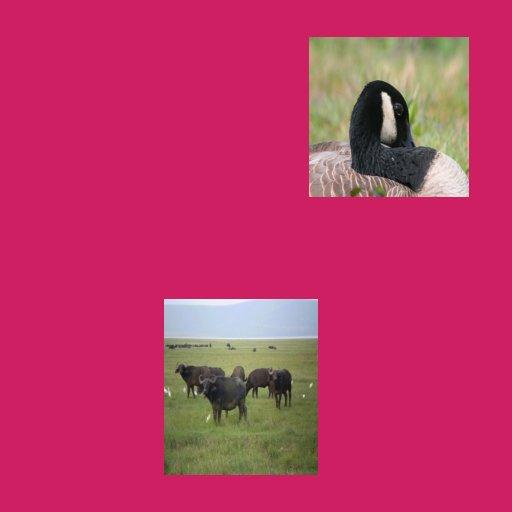
\includegraphics[width=5cm]{x_supple/files/topright1.jpg}} &
\parbox[c]{6cm}{\raggedright\normalsize A blue-toned photograph of a coastal scene with waves. Describe the scene.} &
\raisebox{-0.5\height}{\includegraphics[width=5cm]{example-image-a}} &
\parbox[c]{6cm}{\raggedright\normalsize A warm sunset over a desert canyon with sandstone. What colors are present?} \\

\addlinespace[10pt]

\raisebox{-0.5\height}{\includegraphics[width=5cm]{example-image-a}} &
\parbox[c]{6cm}{\raggedright\normalsize A lush green forest with sunlight filtering through. Identify vegetation types.} &
\raisebox{-0.5\height}{\includegraphics[width=5cm]{example-image-a}} &
\parbox[c]{6cm}{\raggedright\normalsize A purple-tinted cityscape at twilight with neon. Describe the environment.} \\

\addlinespace[10pt]

\raisebox{-0.5\height}{\includegraphics[width=5cm]{example-image-a}} &
\parbox[c]{6cm}{\raggedright\normalsize A lush green forest with sunlight filtering through. Identify vegetation types.} &
\raisebox{-0.5\height}{\includegraphics[width=5cm]{example-image-a}} &
\parbox[c]{6cm}{\raggedright\normalsize A purple-tinted cityscape at twilight with neon. Describe the environment.} \\

\addlinespace[10pt]

\raisebox{-0.5\height}{\includegraphics[width=5cm]{example-image-a}} &
\parbox[c]{6cm}{\raggedright\normalsize A lush green forest with sunlight filtering through. Identify vegetation types.} &
\raisebox{-0.5\height}{\includegraphics[width=5cm]{example-image-a}} &
\parbox[c]{6cm}{\raggedright\normalsize A purple-tinted cityscape at twilight with neon. Describe the environment.} \\
\addlinespace[4pt]

\bottomrule
\end{tabular}
}% end resizebox
\caption{Examples of spatial relation dataset.}
\end{table*}